\section{Discussion sur la situation actuelle en France}

This chapter turns the tools of the two previous ones on the question that
dominates French public finance in 2026: can the dette publique be kept
soutenable, and how can the déficit public be cut without stifling growth? The
first part builds the frame of analysis --- solvabilité as against
soutenabilité; the arithmetic of the ratio dettes/PIB, driven by the gap
$r - g$ between the taux d'intérêt and the taux de croissance and by the solde
primaire; the solde primaire stabilisant; the European and French budget
rules; and the limits of a high debt. The second part asks how to bring
the deficit and the debt down: first whether the debt held by the Eurosystème could simply be cancelled, then
the levers that a 2025 study of the Conseil d'analyse économique (CAE) costs one
by one --- raising revenue, cutting spending and mobilising structural levers.\\

The material is recent and full of numbers: the dates, percentages and tables
are part of what is to be known.

\subsection{Contexte général}

The starting point is historical. En 1944, le \textbf{ratio dettes/PIB}
(\textit{debt-to-GDP ratio}) a atteint des sommets proches de 319~\% du PIB,
mais son remboursement après 1945 (160~\% en 1945) n'a pas résulté d'une
austérité prolongée~: il a reposé sur une forte croissance réelle et une
inflation soutenue sur plusieurs décennies. Les Trente Glorieuses, portées par
la reconstruction, la productivité et la démographie, ont fait baisser le ratio
sans nécessiter de surplus budgétaires continus. L'inflation a réduit la valeur
réelle de la dette, facilitant l'ajustement.\\

La période actuelle est différente. La croissance potentielle est plus basse,
l'inflation reflue et les marges de politique monétaire sont resserrées. Il
devient dès lors plus difficile de laisser l'économie «~faire le travail~» sur
la dette~: il faut des réformes de structure, penser la qualité des dépenses
publiques, la hausse des impôts et taxes, et les priorités d'investissement.\\

Two further facts frame the whole chapter. Historiquement, aucun grand pays
développé n'a réellement remboursé sa dette publique. En réalité, les États ne
cherchent pas tant à rembourser leur dette qu'à la rendre soutenable en suivant
l'évolution du ratio dettes/PIB~: si le PIB croît plus vite que la dette, son
poids relatif diminue mécaniquement. Hence the question the chapter is built
around, answered in its conclusion:

\begin{center}
  \emph{Comment réduire le déficit public et stabiliser la dette publique en
  maintenant la croissance économique~?}
\end{center}

\subsection{Réflexions sur la soutenabilité de la dette publique}

Whether a debt is too high cannot be read off its level. This part separates a
static notion, the capacity to repay today, from a dynamic one, the capacity to
keep the debt under control over time, and then gives the arithmetic that the
dynamic notion rests on.

\subsubsection{La notion de soutenabilité de la dette}

\paragraph{Les spécificités de la contrainte budgétaire publique.}
A State does not face its contrainte budgétaire the way a household or a
firm does. What sets the \textbf{contrainte budgétaire publique}
(\textit{government budget constraint}, CB) apart starts with the notion of
solvabilité.

\begin{definition}[Solvabilité (\textit{solvency})]
  La \textbf{solvabilité} est la capacité financière d'un État à rembourser sa
  dette~: c'est une notion statique (en $t$, a-t-on les actifs suffisants pour
  payer les dettes~?).
\end{definition}

La dette pèse sur le budget public par deux coûts~: 1) celui des intérêts payés,
la \textbf{charge de la dette} (\textit{interest burden}), ou charge d'intérêts~;
2) celui du remboursement de l'emprunt, à la fin. Un État n'a pas les mêmes
contraintes de solvabilité qu'un agent privé, car~:
\begin{itemize}
  \item sa durée de vie est illimitée~: sa CB est intertemporelle. L'enjeu est
    de maîtriser les intérêts payés et d'être capable de faire
    «~\textbf{rouler la dette}~» (\textit{roll over the debt})~; rembourser le
    principal est «~secondaire~» (selon les conditions de marché~!)~;
  \item il a le pouvoir de lever des impôts.
\end{itemize}
As long as the markets lend on acceptable terms the principal is
refinanced rather than repaid, so the burden that really constrains a State is
the interest it pays.

\paragraph{Insolvabilité, défaut de paiement et conséquences.}
When the markets stop believing that a State can pay, the mechanism feeds on
itself. L'\textbf{insolvabilité} (\textit{insolvency}) entraîne une explosion
des taux d'emprunt, puis un cercle vicieux qui empêche tout remboursement de la
dette publique~: c'est la voie du \textbf{défaut de paiement}
(\textit{default}).

\begin{example}[La dette grecque]
  La dette grecque a été jugée insolvable par les marchés à partir de fin 2009.
  Après cela, la Grèce a cessé d'émettre directement sur les marchés primaires,
  et des plans d'aide d'organisations publiques ont pallié le fait qu'elle
  n'émettait plus sur les marchés. D'où le rôle essentiel du comportement des
  créanciers.
\end{example}

\begin{remark}[Formulation du cours]
  «~dette grecque considérée non solvable par les marchés en 2008~».
\end{remark}

Les conséquences de l'insolvabilité sont de trois ordres~:
\begin{itemize}
  \item si un État est insolvable, la communauté internationale de prêteurs peut
    prêter ou annuler tout ou partie de la dette pour éviter une crise majeure et
    la contagion à d'autres pays~;
  \item la \textbf{restructuration de la dette publique} (\textit{public debt
    restructuring})~: allongement de la maturité des dettes, renégociation des
    clauses~;
  \item l'anéantissement de la confiance des investisseurs envers cet État~:
    dépréciation de la valeur des crédits de cet État, d'où une hausse du coût du
    retour sur les marchés financiers (intérêts et primes de risque diverses).
\end{itemize}

Two notions sit behind these consequences: the obligation, the security
through which a State borrows on the marchés primaires and whose terms a
restructuration changes, and the contagion of a crisis from one country to
others.\\

\textbf{Les obligations.}
\begin{definition}[Obligation (\textit{bond})]
  Une \textbf{obligation} est une reconnaissance de dette (part d'un emprunt)
  émise par une entité (l'État, une collectivité locale ou une entreprise). Si
  vous détenez des obligations, vous êtes donc le prêteur (le créancier) de
  l'entité ayant émis ce titre. En échange de ce prêt, vous percevez des
  intérêts. Le taux d'intérêt est connu à l'avance tout comme la durée du prêt
  et la date de versement des intérêts.
\end{definition}
Contrairement aux actions, le versement des intérêts pour le détenteur d'une
obligation n'est pas conditionné à la situation financière de son émetteur, par
exemple aux résultats financiers d'une entreprise.

\begin{example}[Une obligation grecque]
  Quand vous achetez une obligation grecque, vous prêtez de l'argent à la
  Grèce, et en échange l'État s'engage à vous verser un intérêt (le taux de
  7,1~\%) chaque année avant de vous rendre votre mise.
\end{example}

Le vocabulaire des obligations~:
\begin{itemize}
  \item Le \textbf{nominal} (\textit{face value}), ou valeur faciale, ou
    principal, est égal au capital de départ emprunté par l'émetteur de
    l'obligation divisé par le nombre de titres émis. Par exemple, un émetteur
    décide d'emprunter un million d'euros~; ce capital sera divisé en
    différentes coupures, par exemple de 1\,000 euros, pour faciliter les
    échanges sur le marché. Ce montant de 1\,000 euros correspond à la valeur
    nominale de l'obligation.
  \item L'\textbf{échéance} (\textit{maturity}), ou maturité, est la durée de
    vie de l'obligation. Elle peut correspondre à la date à laquelle le
    détenteur de l'obligation se voit rembourser le montant intégral du nominal,
    c'est-à-dire le capital emprunté par l'émetteur~: on parle alors de
    \textbf{remboursement du capital in fine} (\textit{bullet repayment}). Ce
    remboursement peut aussi être régulier et se réaliser par un
    \textbf{amortissement constant} (\textit{constant amortisation}) --- la même
    part de capital est remboursée à chaque versement, si bien que les
    versements décroissent --- ou par \textbf{annuités constantes}
    (\textit{constant annuities}) --- le versement total, intérêts et capital,
    est constant. L'échéance moyenne d'une obligation est de dix ans.
  \item Le coupon correspond au versement périodique d'un intérêt au détenteur
    de l'obligation. Selon la nature de l'obligation, le versement des intérêts
    peut être régulier (généralement tous les ans) ou intervenir in fine,
    c'est-à-dire à l'échéance. De même, le taux d'intérêt versé peut être un
    \textbf{taux fixe} (\textit{fixed rate}), et le revenu de l'intérêt perçu
    périodiquement est constant, ou un \textbf{taux variable}
    (\textit{variable rate}), qui varie en fonction des taux du marché.
\end{itemize}

\begin{remark}[Formulation du cours]
  «~amortissement constant (chaque versement comprend une part identique de
  coupon et de capital) ou par annuités constantes (le capital remboursé est
  constant à chaque versement)~».
\end{remark}

\textbf{La contagion.} The first consequence above, the contagion to other
countries, is a mechanism of its own.

\begin{definition}[Contagion financière (\textit{financial contagion})]
  Le mécanisme de \textbf{contagion financière} est un \textbf{effet domino}
  (\textit{domino effect}), où la panique des investisseurs se propage d'un pays
  fragile à un autre, même si leurs situations de départ sont différentes.
\end{definition}

\begin{figure}[h!]
  \centering
  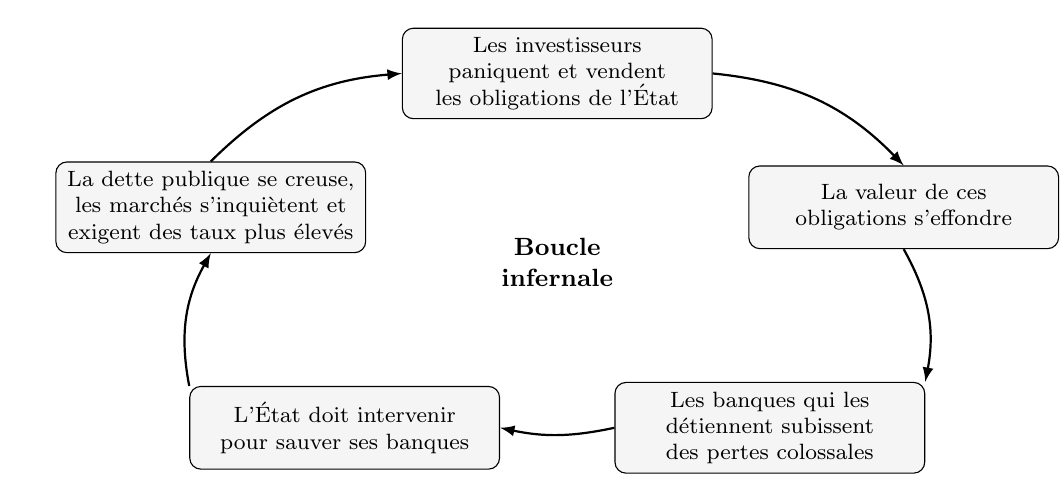
\begin{tikzpicture}[>=latex, every node/.style={font=\footnotesize},
      etape/.style={draw, rounded corners, align=center, text width=3.7cm,
        minimum height=1.05cm, fill=gray!8,
        execute at begin node={\hyphenpenalty=10000\relax}}]
    \node[etape] (a) at (0,2.5) {Les investisseurs paniquent et vendent les
      obligations de l'État};
    \node[etape] (b) at (4.4,0.8) {La valeur de ces obligations s'effondre};
    \node[etape] (c) at (2.7,-2.0) {Les banques qui les détiennent subissent
      des pertes colossales};
    \node[etape] (d) at (-2.7,-2.0) {L'État doit intervenir pour sauver ses
      banques};
    \node[etape] (e) at (-4.4,0.8) {La dette publique se creuse, les marchés
      s'inquiètent et exigent des taux plus élevés};
    \draw[->, thick] (a.east) to[bend left=20] (b.north);
    \draw[->, thick] (b.south) to[bend left=20] (c.north east);
    \draw[->, thick] (c.west) to[bend left=12] (d.east);
    \draw[->, thick] (d.north west) to[bend left=20] (e.south);
    \draw[->, thick] (e.north) to[bend left=20] (a.west);
    \node[font=\small\bfseries, align=center] at (0,0.1) {Boucle\\infernale};
  \end{tikzpicture}
  \caption*{\small La boucle infernale entre les banques et les États. Each
    arrow is one step of the mechanism traced in the example below; the loop closes because
    the rescue of the banks raises the very dette publique whose obligations
    they hold, and the markets then demand still higher rates.}
\end{figure}

\begin{example}[La contagion de la crise grecque à la zone euro]
  Lorsque les investisseurs ont réalisé que la Grèce risquait la faillite, ils
  ont immédiatement cherché quels étaient les prochains maillons faibles de la
  zone euro. L'Espagne souffrait alors de l'éclatement d'une bulle immobilière
  massive et d'un chômage record~; l'Italie traînait une dette publique
  historique très élevée (bien que son déficit budgétaire annuel soit mieux
  maîtrisé).\\

  Les banques espagnoles et italiennes possédaient d'énormes quantités
  d'obligations de leur propre État. Quand les investisseurs paniquent, ils
  vendent les obligations italiennes et espagnoles, et la valeur de ces
  obligations s'effondre. En conséquence, les banques qui détiennent ces titres
  subissent des pertes colossales et affichent une santé financière fragile~;
  l'État doit intervenir pour sauver ses banques, ce qui creuse encore plus sa
  propre dette publique et inquiète davantage les marchés. C'est ce qu'on
  appelle la \textbf{boucle infernale} (\textit{doom loop}) entre les banques
  et les États.\\

  Pour compenser ce nouveau risque, les investisseurs ont exigé des taux
  d'intérêt de plus en plus élevés pour prêter à Rome ou à Madrid~: emprunter
  est devenu hors de prix pour l'Italie et l'Espagne, menaçant de les asphyxier
  financièrement, exactement comme la Grèce. Si l'Italie
  (3\textsuperscript{e} économie de la zone euro) avait fait faillite, elle
  aurait entraîné dans sa chute les banques françaises et allemandes qui lui
  avaient prêté de l'argent, menaçant de faire exploser l'euro tout entier.\\

  Le domino ne s'est arrêté qu'en juillet 2012, grâce à la célèbre déclaration
  de Mario Draghi, alors président de la BCE~: «~La BCE est prête à faire tout
  ce qu'il faudra (\emph{whatever it takes}) pour préserver l'euro. Et
  croyez-moi, ce sera suffisant.~» En garantissant que la banque centrale
  rachèterait si nécessaire les dettes des pays attaqués, il a calmé la
  spéculation du jour au lendemain. La BCE a en effet créé un programme d'achat
  de titres publics sur le marché secondaire, appelé Outright Monetary
  Transactions (OMT), pour des quantités illimitées, qui a concrétisé le
  «~whatever it takes~» de Mario Draghi.
\end{example}

\paragraph{La notion de soutenabilité = approche dynamique de la dette.}
Where solvabilité looks at a single date, soutenabilité looks at the path.

\begin{definition}[Soutenabilité (\textit{sustainability})]
  La \textbf{soutenabilité} est la capacité d'un pays à assurer le service de
  sa dette sans compromettre sa croissance à long terme (sans hausse excessive
  de la pression fiscale ou baisse des services publics qui étoufferaient la
  croissance et provoqueraient des troubles sociaux)~: c'est une notion de
  trajectoire «~viable~» de la dette, c'est-à-dire de contrôle en situation
  économique «~normale~».
\end{definition}

\begin{definition}[Non soutenabilité (\textit{unsustainability})]
  Il y a \textbf{non soutenabilité} quand la dette ou son service atteint un
  niveau tel que la restructuration est la seule solution possible (on
  renégocie les termes de la dette avec les créanciers, voire une réduction
  partielle, un allongement).
\end{definition}

La soutenabilité vaut aussi pour la trajectoire de réduction (des déficits et de
la dette)~: pas de trajectoire trop sévère, qui provoquerait une crise. Définir
la soutenabilité de la dette publique procède donc de deux questions~:
\begin{enumerate}
  \item quelle est la trajectoire de long terme de la dette~?
  \item cette trajectoire rencontre-t-elle à un moment une condition de rupture,
    la rendant insoutenable~?
\end{enumerate}
The rest of this subsection answers the first question with the dynamics of the
ratio dettes/PIB; the limits of a high debt, further on, answer the second.

\paragraph{La trajectoire de la dette publique.}
The debt dynamics need a handful of symbols, all defined on the same date
convention.

\begin{notation}
  Les notations de la trajectoire de la dette~:
  \begin{itemize}
    \item $D_{t+1}$~: montant de la dette publique en $t+1$~; $D_t$~: montant
      de la dette publique en $t$.
    \item $SP_{t+1}$~: montant du \textbf{solde primaire}
      (\textit{primary balance}) en $t+1$, c'est-à-dire le solde effectif hors
      charge d'intérêts~; $SP > 0$~: excédents, $SP < 0$~: déficits.
    \item $r$~: taux d'intérêt nominal, le \textbf{taux d'intérêt apparent de la
      dette} (\textit{implicit interest rate on the debt}).
    \item $g$~: taux de croissance nominale.
  \end{itemize}
\end{notation}

Le \textbf{solde primaire structurel} (\textit{structural primary balance}) en
retire aussi la part conjoncturelle~: il est calculé hors charge d'intérêts et
hors aléas conjoncturels.

\begin{remark}[Formulation du cours]
  «~$SP_{t+1}$ = montant du solde primaire structurel en $t+1$~».
\end{remark}

To strip out the cycle one needs a benchmark for normal output. On évalue le
\textbf{PIB potentiel} (\textit{potential GDP})~: c'est le niveau de production
réalisable sans tensions, le niveau du PIB qui serait constaté si celui-ci
augmentait toujours au même rythme sur un cycle économique~; ce rythme est la
\textbf{croissance potentielle} (\textit{potential growth}). L'écart entre le PIB
effectif et le PIB potentiel est désigné par l'expression
\textbf{écart de production} (\textit{output gap}).\\

The rate $r$ is not the rate the market quotes today. Le taux apparent (taux
d'intérêt moyen sur le stock de dette en cours) diffère du \textbf{taux
souverain} (\textit{sovereign yield}), le taux actuel sur le marché. L'impact
d'une hausse des taux d'intérêt souverains sur le taux d'intérêt apparent est
progressif~: la charge d'intérêts de la dette publique n'augmente pas
immédiatement dès que les taux souverains varient à la hausse. Only the debt
issued or refinanced after the rise pays the new rate, so the average rate on
the whole stock catches up slowly.

\paragraph{Facteurs d'évolution de la dette.}
On peut écrire
\[ D_{t+1} = D_t(1+r) - SP_{t+1}, \]
that is, next year's debt is this year's debt plus its interest, less the solde
primaire. Dividing by $\text{PIB}_{t+1} = \text{PIB}_t(1+g)$ gives the ratio
\[ \frac{D_{t+1}}{\text{PIB}_{t+1}} = \frac{D_t}{\text{PIB}_t} \times
   \frac{1+r}{1+g} - \frac{SP_{t+1}}{\text{PIB}_{t+1}}, \]
soit, avec $d_t = D_t/\text{PIB}_t$ et $sp_{t+1} = SP_{t+1}/\text{PIB}_{t+1}$,
\[ d_{t+1} = d_t \times \frac{1+r}{1+g} - sp_{t+1}. \]
Pour $r$ et $g$ petits, $\dfrac{1+r}{1+g} \approx 1 + r - g$, d'où
\[ d_{t+1} \approx d_t(1 + r - g) - sp_{t+1}, \qquad
   \Delta d_t = d_{t+1} - d_t \approx d_t(r - g) - sp_{t+1}. \]

Bilan~: l'évolution de la dette dépend de $sp$, $r$ et $g$. This answers the
first of the two questions of soutenabilité. Two regimes follow:
\begin{enumerate}
  \item L'\textbf{effet boule de neige} (\textit{snowball effect})~: si
    $r > g$, $d_t$ augmente même sans déficit~; il faut un excédent, au prix
    d'une austérité. «~Si le taux de croissance de l'économie est inférieur au
    taux d'intérêt réel, même un faible déficit primaire peut entraîner une
    dynamique explosive de la dette publique.~» (Olivier Blanchard, 2017.) The
    quotation speaks of the real rate while $r$ here is nominal; this changes
    nothing, because $r - g$ has the same sign whether both are taken in real
    terms or both in nominal terms. In chapter 7 the same words describe the
    successive rounds of spending of the effet multiplicateur; here, as in the
    rest of this chapter, they name a debt that grows on its own interest
    faster than the economy.
  \item Si $g > r$, le ratio dette/PIB peut baisser même avec un déficit
    primaire «~modéré~».
\end{enumerate}

\paragraph{Soutenabilité de la dette~: rôle de $r - g$ et de $sp$.}
The sign of $r - g$ decides which regime a country is in.
\begin{itemize}
  \item Quand $r - g$ est négatif, un pays très endetté peut paraître soutenable
    quels que soient ses choix budgétaires~: des taux réels négatifs rendent
    $r - g$ favorable, indépendamment des choix budgétaires. Mais en France
    $r - g$ n'est devenu négatif qu'au milieu des années 2010 (hors 2020), et en
    Italie il est resté le plus souvent positif jusqu'en 2020.
  \item Quand $r - g$ est proche de zéro --- c'est la configuration de début
    2026 pour la plupart des économies avancées ---, le poids de la CB, qui
    avait disparu pendant une décennie entière, est rétabli~: chaque point de
    déficit primaire pèse désormais directement sur la trajectoire du ratio
    dette/PIB, ce qui pousse à la hausse la prime de risque sur la dette et
    exige un solde primaire en excédent pour stabiliser la dette.
\end{itemize}
Comparing the taux d'intérêt apparent with the croissance nominale in France
since 1950 shows the regimes in turn: du milieu des années 1980 au milieu des années
2010, $r - g$ est le plus souvent positif en France (effet boule de neige), puis
négatif.

\subsubsection{Comment stabiliser la dette~?}

\paragraph{Solde primaire stabilisant.}
Stabilising the debt means holding the ratio, not the amount, constant. La
\textbf{condition de stabilisation} (\textit{stabilisation condition}) s'écrit
$d_{t+1} - d_t = 0$. Setting $\Delta d_t = 0$ in the dynamics above gives the
solde primaire that does it.

\begin{definition}[Solde primaire stabilisant (\textit{debt-stabilising primary balance})]
  Le \textbf{solde primaire stabilisant} (SPS) est le solde primaire qui
  stabilise le ratio d'endettement~:
  \[ sps_{t+1} = d_t(r - g). \]
\end{definition}

Si $sp > sps$, l'endettement baisse. Si $sp < sps$, la dette augmente, même si
$r < g$, car il n'y a pas de compensation suffisante par le solde. When
$r < g$ the solde primaire stabilisant is negative, so a déficit primaire can
be afforded, but only up to that bound.\\

Three questions test the formula.

\begin{example}[Si $r = g$~?]
  With $r = g$ exactly, $sps_{t+1} = d_t(r - g) = 0$: a solde primaire of zero
  holds the ratio, any déficit primaire raises it and any excédent primaire
  lowers it. This is the case of $r - g$ close to zero above. The weight of the
  CB is back, and every point of déficit primaire bears directly on the ratio
  dettes/PIB. Since each such point also pushes up the prime de risque, and with
  it $r$, stabilising the debt then calls for a solde primaire en excédent, as
  that bullet concludes.
\end{example}

\begin{example}[Si la dette est stabilisée à 500~\% du PIB~?]
  With $d_t = 5$ the formula gives $sps_{t+1} = 5(r - g)$: every point by which
  $r$ exceeds $g$ calls for an excédent primaire of five points of PIB, year after
  year. The formula can stabilise any ratio on paper; whether a country can
  actually run such an excédent is the question of the excédent primaire
  maximal, taken up with the limits of a high debt below.
\end{example}

\begin{example}[Limites de cette formule~?]
  Bilan~: la définition de la soutenabilité ne permet pas de juger d'un niveau
  excessif d'endettement. The formula says at which solde primaire a given
  ratio stops rising; it says nothing about whether that ratio is too high,
  nor about the threshold at which creditors stop lending. Those limits are the
  subject of the questions on a high debt below.
\end{example}

\paragraph{Solde public, solde primaire et soldes stabilisants de 2005 à 2025.}
The same reasoning applies to the solde public, interest included. Solde
public = solde primaire $-$ charge d'intérêts de la dette (soit déficit public =
déficit primaire + charge d'intérêts).

\begin{remark}[Formulation du cours]
  «~Solde public = solde primaire + charge d'intérêt de la dette~».
\end{remark}

Pour stabiliser la dette, il faut donc soit un \textbf{excédent stabilisant}
(\textit{debt-stabilising surplus}), soit un \textbf{déficit stabilisant}
(\textit{debt-stabilising deficit}). Which of the two depends on the sign of
$r - g$. France's balances from 2005 to 2025 show both cases. In 2020, when the
PIB nominal fell, stabilising the debt required an excédent stabilisant; in
2021, with the rebound of the croissance nominale, a déficit stabilisant
sufficed.

\subsubsection{Procédure de déficits excessifs et engagements de la France}

\paragraph{Les cadres juridiques d'encadrement de la dette.}
The European frame comes first. Le traité sur la stabilité, la coordination et
la gouvernance (TSCG), de 2012, pose trois règles~:
\begin{itemize}
  \item l'objectif de moyen terme (OMT), fixé tous les 3 ans, est la cible de
    solde structurel pour chaque pays~;
  \item la \textbf{règle d'or} (\textit{golden rule}) en Europe est une
    obligation qui limite le déficit budgétaire structurel à 0,5~\% du PIB (ou
    1~\% pour certains pays si la dette est très faible, c'est-à-dire
    inférieure à 60~\% du PIB)~;
  \item l'Union européenne impose aux États membres d'inscrire une règle
    d'équilibre budgétaire dans leur droit national, de préférence au niveau
    constitutionnel.
\end{itemize}
La réforme de 2024 du cadre budgétaire de l'UE (règlement 2024/1263), distincte
du TSCG, y ajoute deux règles chiffrées~:
\begin{itemize}
  \item le solde primaire structurel doit s'améliorer de 0,4 point de PIB par an
    (0,25 point si l'ajustement est prolongé) jusqu'à un déficit structurel de
    1,5~\% du PIB~;
  \item la dette doit baisser en moyenne d'au moins 1 point de PIB par an
    au-delà de 90~\% du PIB, et de 0,5 point entre 60 et 90~\%.
\end{itemize}

\begin{remark}[Formulation du cours]
  Rattachées au TSCG (2012)~: «~Le déficit primaire structurel doit diminuer
  d'au moins 0,4 point de PIB chaque année tant que le déficit structurel reste
  supérieur à 1,5~\% du PIB~» et «~Les États placés sous procédure de déficit
  excessif doivent réduire la dette d'environ 1~\%/an si elle dépasse 90~\% du
  PIB, et d'environ 0,5~\% par an si elle se situe entre 60~\% et 90~\% du
  PIB~».
\end{remark}

France then wrote this requirement into its own law, without touching the
Constitution. La France a choisi de ne pas modifier sa Constitution~; à la
place, elle a transposé cette obligation via la \textbf{loi organique du 17
décembre 2012 relative à la programmation et à la gouvernance des finances
publiques} (\textit{Organic Law on the Programming and Governance of
Public Finances}, LOPGFP), qui~:
\begin{itemize}
  \item impose le vote de \textbf{lois de programmation des finances publiques}
    (\textit{public finance programming laws}, LPFP) définissant une
    trajectoire pluriannuelle vers l'équilibre (2023-2027)~;
  \item a créé le \textbf{Haut Conseil des finances publiques}
    (\textit{High Council of Public Finances}, HCFP), un organisme indépendant chargé
    de vérifier si les budgets de l'État dévient ou non de cette trajectoire, et
    a introduit un mécanisme de correction.
\end{itemize}
La règle d'or budgétaire en France, qui impose des finances équilibrées, ne
concerne que les collectivités territoriales (communes, départements, régions).
L'État central, lui, conserve le droit de voter un budget en déficit.

\paragraph{La dette française~: troisième ratio d'endettement en Europe mais «~attractive sous surveillance~».}
Where France stands, and what it has committed to:
\begin{itemize}
  \item Au premier trimestre 2025, la France se situe au troisième rang des pays
    de l'Union monétaire pour le ratio dettes publiques/PIB (114,1~\%),
    derrière la Grèce et l'Italie. L'Allemagne est proche de 60~\%, l'Espagne
    autour de 103,5~\%, et la moyenne de la zone euro avoisine 88~\%~: ce
    contraste témoigne de trajectoires budgétaires et de choix politiques
    divergents étalés sur vingt ans.
  \item La réactivation du cadre budgétaire européen s'accompagne désormais de
    \textbf{plans d'ajustement pluriannuels} (\textit{multiannual adjustment
    plans}) pays par pays. Pour la France, l'équation consiste à cibler l'effort
    sur les dépenses les moins productives, à sanctuariser l'investissement utile
    à la croissance potentielle et à sécuriser les recettes tout en préservant la
    compétitivité.
  \item La France est sous une procédure de déficit excessif depuis juillet 2024
    et doit limiter la progression nette de ses dépenses publiques à 0,8~\% en
    2025 et 1,2~\% en 2026. Sur la base des données fournies par la France fin
    octobre 2025, la Commission européenne juge que Paris respecte le chemin
    défini par la procédure de déficit excessif.
  \item Dans ses prévisions de printemps 2026, la Commission s'attend à un
    déficit de 5,1~\% du PIB en 2026, puis de 5,7~\% en 2027, et à une dette de
    118,1~\% du PIB en 2026 et de 120,2~\% en 2027. C'est une trajectoire
    distincte de celle du plan français (le plan budgétaire et structurel à
    moyen terme, PSMT, d'octobre 2024), qui vise à ramener le déficit public sous
    3~\% du PIB d'ici 2029 --- 2,8~\% en 2029 ---, la dette culminant vers
    116,5~\% en 2027 puis revenant à 115,8~\% en 2029.
  \item Malgré un ratio d'endettement élevé, il y a une demande des
    investisseurs, mais à un coût supérieur, et pas de revente massive~: c'est
    un capital de confiance. Mais 57~\% de la dette est
    détenue par des non-résidents, et récemment par une part accrue de hedge
    funds (fonds spéculatifs), pour environ 60~Md€.
\end{itemize}

\subsubsection{Dette~: un fardeau intergénérationnel~?}

Whether the debt passes a charge on to the next generations depends on what it
pays for. La dette publique est-elle un \textbf{fardeau intergénérationnel}
(\textit{intergenerational burden})~?
\begin{itemize}
  \item \textbf{oui}, si elle résulte d'un endettement destiné à des dépenses
    courantes non productives ou à des déficits structurels (financer un trou
    dans les finances publiques créé par des cadeaux fiscaux ou par des dépenses
    discutables)~: c'est la dette sociale, laissée aux générations futures~;
  \item \textbf{non}, si elle finance des investissements qui génèrent des
    revenus à long terme et qui soutiennent la croissance (investissements dans
    le domaine de l'infrastructure, de l'éducation, de la recherche, de la
    santé).
\end{itemize}

\subsubsection{Y a-t-il des limites à une dette élevée~?}

This answers the second question of soutenabilité, whether the trajectory meets
a breaking point. First, what counts as a high debt? Le SPS peut être élevé tant
que la trajectoire est soutenable et tant que la dette finance des
investissements de long terme (défense, innovation…). Mais le contexte
économique joue aussi un rôle, à travers plusieurs risques~:
\begin{itemize}
  \item un risque de perte de contrôle de la dette, par l'effet boule de neige
    (avec $r > g$)~: hausse permanente du poids de la dette~; il faut dégager un
    $sps$ excédentaire qui croît~;
  \item un risque de debt overhang~: plus la dette se stabilise à un niveau
    élevé, plus ce risque augmente, car il n'y a plus de soutien possible par la
    dépense publique en cas de nouveau choc~;
  \item il est impossible de déterminer le niveau maximal de stabilisation du
    seuil d'endettement qui déclenche une crise des finances publiques
    (c'est-à-dire qui crée une anticipation de défaut de paiement par les
    investisseurs), et il existe un \textbf{excédent primaire maximal}
    (\textit{maximum primary surplus}) propre à chaque pays. Il ne suffit donc
    pas de pouvoir stabiliser la dette~; encore faut-il qu'elle puisse être
    stabilisée à un niveau qui permette de garder la confiance des créanciers
    de l'État~;
  \item un risque de perte de \textbf{souveraineté budgétaire}
    (\textit{fiscal sovereignty})~: un État en défaut de paiement peut faire
    appel à des institutions internationales qui jouent le rôle de prêteur en
    dernier ressort, comme le Fonds monétaire international (FMI), mais en
    contrepartie de mesures de rééquilibrage des comptes publics souvent
    douloureuses pour la population~;
  \item un risque récessionniste~: pour contrôler l'inflation, si de nombreux
    pays sont en déficits excessifs récurrents, la BCE peut augmenter encore plus
    les taux d'intérêt.
\end{itemize}

\subsubsection{Les défis liés au maintien d'un solde primaire $sp > 0$}

Even a country that needs an excédent primaire finds it hard to keep one, for four
reasons:
\begin{enumerate}
  \item la volatilité des revenus face à la rigidité des dépenses publiques
    (retraite, santé), moins ajustables à court terme~: d'où des déficits
    persistants en période de faible croissance~;
  \item la pression sur les politiques pour augmenter les dépenses et baisser
    les impôts (cycle électoral), et la résistance aux réformes (par exemple, la
    hausse de l'âge de la retraite)~;
  \item si le niveau des dettes est élevé, le poids des intérêts rend $sp$
    faible ou négatif~;
  \item l'évolution démographique~: le vieillissement augmente la pression sur
    les coûts et réduit la croissance potentielle.
\end{enumerate}

\subsection{Comment réduire le déficit et la dette~?}

The second part looks for ways out. The tempting shortcut, cancelling the part
of the debt held by the central bank, is examined first and turned down; the
rest of the part follows a costed study of what revenue, spending and
réformes structurelles could deliver.

\subsubsection{Peut-on annuler la dette publique détenue par l'Eurosystème~?}

Some background first. La BCE a racheté sur le marché secondaire des
obligations souveraines (et privées) pour augmenter la soutenabilité de la dette
européenne dans les années 2015-2022~; ces avoirs sont en réduction progressive
depuis. En septembre 2025, l'Eurosystème détenait 19,9~\% de la dette publique
française~; la Banque de France (BdF) en détenait 488~Md€ (au coût amorti) au
30 juin 2026.\\

The case for cancelling runs as follows. L'État et la Banque de France forment,
d'un point de vue consolidé, la même entité publique~: annuler la dette
reviendrait à «~effacer une ardoise que l'on a envers soi-même~». L'effacement
des titres de dette entraînerait une baisse instantanée du ratio dettes/PIB.

\paragraph{Mais de nombreuses limites/contraintes…}
The answer is nonetheless no, for several reasons.
\begin{itemize}
  \item L'interdiction juridique de \textbf{«~monétiser~»}
    (\textit{monetise}) une dette, c'est-à-dire de financer directement
    (gratuitement) l'État. L'article 123, paragraphe 1, du traité sur le
    fonctionnement de l'Union européenne (TFUE) dispose~: «~Il est interdit à la
    Banque centrale européenne et aux banques centrales des États membres […]
    d'accorder des découverts ou tout autre type de crédit aux institutions,
    organes ou organismes de l'Union, aux administrations centrales, aux
    autorités régionales ou locales, aux autres autorités publiques, aux autres
    organismes ou entreprises publics des États membres~; l'acquisition directe,
    auprès d'eux, par la Banque centrale européenne ou les banques centrales
    nationales, des instruments de leur dette est également interdite.~»
    Exception~: des cas exceptionnels (situation de menace), avec l'accord de
    tous les autres pays de l'Union économique et monétaire (UEM).
  \item La hausse des risques sur les pays restants endettés auprès de la BCE~:
    risque de contagion des annulations, remise en cause de la crédibilité de la
    BCE et risque d'inflation galopante, et finalement remise en cause de la
    crédibilité de la zone euro.
  \item La dette est «~rarement remboursée~»~: elle «~roule~». L'annulation ne
    permet donc pas de récupérer des fonds pour investir~; son seul avantage est
    une baisse temporaire du montant de la dette et du déficit, en supprimant des
    intérêts. Tant qu'il y a déficit avec une croissance molle, cela ne change
    pas la dynamique de la dette.
  \item Une volonté affichée de ne pas honorer une partie de la dette publique
    risquerait d'accroître immédiatement les taux exigés pour financer la
    France.
  \item L'envoi d'un signal négatif sur la gestion des déficits, qui encourage à
    ne pas maîtriser la dette.
\end{itemize}

The last limit concerns the «~circuit fermé~» that links the State and the
Banque de France. Dans ce mécanisme, la contrepartie des titres de dette
rachetés est une hausse des réserves excédentaires des banques commerciales,
rémunérées au taux de la facilité de dépôt.

\begin{remark}[Formulation du cours]
  «~Contrepartie des titres de dette = hausse des réserves sur les dépôts
  obligatoires rémunérés des banques commerciales~».
\end{remark}

Les limites actuelles du mécanisme de «~circuit fermé~» sont les suivantes~:
\begin{itemize}
  \item avantage de la détention par la BdF~: les titres ne circulent pas sur les
    marchés secondaires et échappent aux pressions spéculatives~;
  \item mais le rachat d'obligations souveraines se fait contre de la monnaie
    banque centrale versée sur les comptes des banques commerciales, rémunérée au
    taux des dépôts~: si les taux d'intérêt montent pour lutter contre
    l'inflation, le coût augmente~;
  \item historiquement (période de taux bas), l'État versait des intérêts à la
    Banque de France~; celle-ci réalisait un bénéfice et le reversait en grande
    partie à l'État sous forme de dividendes, ce qui constituait une recette
    publique. Comptablement, la dépense (intérêts) était donc neutralisée par la
    recette (dividendes), limitant l'impact réel sur le déficit~;
  \item aujourd'hui (depuis la hausse des taux directeurs), ce mécanisme vertueux
    a disparu. La Banque de France doit désormais rémunérer très cher les
    réserves que les banques commerciales déposent chez elle (au taux de la
    facilité de dépôt). Les intérêts que lui verse l'État servent donc à payer
    les banques privées. La Banque de France ne dégage plus de bénéfices et ne
    verse plus de dividendes à l'État, ce qui rend le poids de ces intérêts bien
    réel pour le déficit public~; la BdF a donc besoin de ces taux. The rates
    meant are the interest the State pays it, which now funds the remuneration
    of the reserves.
\end{itemize}

\subsubsection{L'étude du CAE sur les leviers de stabilisation de la dette}

There is no shortcut, then: the debt has to be stabilised by the budget itself.
The rest of the chapter follows the CAE's costing of the three levers, set out
in the tables below.

\paragraph{Obligation de bâtir une trajectoire soutenable et crédible de stabilisation puis de réduction de la dette.}
The study sets out its aim and its working assumptions.
\begin{itemize}
  \item Objectif~: réduire le déficit afin de garantir la soutenabilité de la
    dette et la crédibilité financière du pays, tout en évitant une
    consolidation trop rapide susceptible de freiner la croissance et l'emploi.
  \item Hypothèses~: remontée des taux des obligations souveraines à 10 ans
    (hausse de la charge d'intérêts) et prise en compte de la dynamique
    tendancielle des finances publiques (progression des dépenses plus rapide
    que celle des recettes au cours des prochaines années).
  \item Durée de consolidation optimale~: un scénario central de six ans. Il est
    en ligne avec les règles budgétaires européennes~; l'effort initial est de
    0,9~\% du PIB, soit 27~Md€ en 2026~; il permet de ramener le déficit public
    sous 3~\% du PIB en 2029.
\end{itemize}

\paragraph{Résultats de l'étude.}
The size of the effort is measured by a single quantity.

\begin{definition}[Impulsion budgétaire (\textit{fiscal impulse})]
  L'\textbf{effort budgétaire primaire structurel} (\textit{structural primary
  fiscal effort}) d'une année à l'autre est l'\textbf{impulsion budgétaire}~;
  elle est négative en période de consolidation et positive en période
  d'expansion budgétaire.
\end{definition}

\begin{itemize}
  \item L'impulsion budgétaire totale est estimée à 112~Md€ pour stabiliser la
    dette, avec un effort optimal de 27~Md€ la première année (hors effort
    relatif au tendanciel). Tant que cet effort n'est pas réalisé, la dette
    augmente (sauf croissance forte).
  \item L'étude identifie 170 mesures, avec leurs économies potentielles~:
    108~Md€ issus des dépenses, 111~Md€ issus des recettes et 45~Md€ issus de
    \textbf{réformes structurelles} (\textit{structural reforms}), c'est-à-dire
    de capacités à augmenter les recettes fiscales sans hausse des impôts (par
    exemple, lutter contre la fraude fiscale).
  \item Plusieurs solutions alternatives sont possibles pour consolider
    l'effort. Aucune option n'est neutre économiquement et socialement~: les
    finances publiques constituent un champ de bataille des luttes sociales.
\end{itemize}
The three amounts are the totals of the three tables that follow, one per lever:
108~Md€ for spending, 111,4~Md€ for revenue and 45,1~Md€ for the réformes
structurelles. Together they exceed the effort required, which is what leaves room
for choice among them.

\paragraph{Le déficit primaire français est surtout structurel.}
Before choosing levers one must know what kind of deficit is to be closed.\\

\begin{table}[h!]
  \centering
  \small
  \begin{tabular}{@{}lr@{}}
    \toprule
    Type de déficit & valeur (\% du PIB) \\
    \midrule
    Déficit public & 5,4 \\
    \quad dont charge de la dette & 2,2 \\
    \quad dont déficit primaire & 3,2 \\
    \qquad dont déficit primaire structurel & 2,7 \\
    \qquad dont déficit primaire conjoncturel
      ($0{,}57 \times$ écart de production de $-0{,}8$ point) & 0,5 \\
    \bottomrule
  \end{tabular}
  \caption*{\small Décomposition du déficit primaire estimé en 2025. The
    déficit public is the déficit primaire plus the charge de la dette
    ($5{,}4 = 3{,}2 + 2{,}2$); the cyclical part of the déficit primaire is the
    écart de production multiplied by the coefficient $0{,}57$.}
\end{table}

Le déficit primaire structurel pèse environ 85~\% (84,4~\%) du déficit primaire
total, et le \textbf{déficit conjoncturel} (\textit{cyclical deficit}) 15,6~\%.
Bilan~: la quasi-totalité du déficit primaire français provient de déséquilibres
permanents et fondamentaux entre les dépenses de fonctionnement des
administrations et leurs recettes fiscales courantes, et non d'un simple
accident lié aux cycles économiques. A deficit of this kind will not close by
itself when growth returns: it has to be closed by decisions on revenue and
spending.

\subsubsection{Augmenter les recettes}

The first lever is revenue. Les sources de recettes les plus rentables sont la
modification des impôts sur les revenus et sur les patrimoines. The measures
are of two kinds. Les \textbf{dépenses fiscales} (\textit{tax expenditures})~:
annuler une exonération réduit la dépense fiscale. Une recette fiscale, elle,
vient augmenter les PO. A dépense fiscale is revenue the State forgoes through
an exemption, so removing one raises revenue without creating a new tax; the
table marks each measure as one or the other.\\

\begin{center}
\begin{minipage}{\textwidth}
  \centering
  \footnotesize
  \begin{tabularx}{\textwidth}{@{}l>{\raggedright\arraybackslash}Xrr@{}}
    \toprule
    & Recettes & PO 2024 & 2026 \\
    \midrule
    & \textbf{Impôts sur le revenu (y compris CSG et CRDS)} & \textbf{268,0} & \textbf{38,2} \\
    R & Augmenter le taux de prélèvement forfaitaire unique (PFU) de 30~\% à 33~\%\textsuperscript{*} & & 1,2 \\
    R & Augmenter d'un point le taux d'IR pour chaque tranche (sauf celle à 0~\%)\textsuperscript{*} & & 6,8 \\
    R & Augmenter d'un point le taux de CSG & & 14,6 \\
    R & Geler l'indexation du barème de l'IR sur l'inflation & & 1,8 \\
    R & Plafonner le bénéfice du quotient conjugal pour les couples mariés ou pacsés ayant les plus hauts revenus (à 10\,000~€) & & 1,1 \\
    R & Supprimer les demi-parts de quotient familial qui ne correspondent pas à des charges effectives & & 2,9 \\
    R & Aligner l'ensemble de la tranche imposée à 8,3~\% de CSG sur celle des actifs imposée à 9,2~\% & & 1,3 \\
    DF & Supprimer les niches fiscales des revenus du capital (assurance-vie, épargne logement) & & 0,9 \\
    DF & Supprimer l'abattement fiscal de 10~\% sur le calcul du revenu fiscal de référence des retraités & & 4,8 \\
    DF & Supprimer l'exonération d'IR accordée à la rémunération des heures supplémentaires et complémentaires & & 1,8 \\
    DF & Supprimer la réduction d'impôt sur le revenu à raison des investissements productifs en outre-mer\textsuperscript{*} & & 0,3 \\
    DF & Limiter le plafond de don du taux normal de la réduction d'IR à 2\,000~€ & & 0,4 \\
    DF & Réformer le crédit d'impôt au titre de l'emploi d'un salarié à domicile & & 0,4 \\
    \midrule
    & \textbf{Impôts sur le patrimoine (DMTO, DMTG, taxes foncières, IFI, taxe d'habitation)} & \textbf{86,9} & \textbf{38,4} \\
    R & Restaurer la taxe d'habitation sur les résidences principales & & 21,8 \\
    R & Supprimer les abattements sur les plus-values immobilières pour durée de détention & & 3,6 \\
    R & Rétablir l'ISF selon les mêmes modalités qu'avant sa suppression & & 5,0 \\
    DF & Taxation de l'héritage~: supprimer ou réviser les dispositifs d'allègement & & 8,0 \\
    \midrule
    & \textbf{Impôt sur les sociétés} & \textbf{57,4} & \textbf{4,8} \\
    R & Augmenter le taux d'imposition sur les sociétés (IS) de 25~\% à 33,5~\%\textsuperscript{*} & & 4,4 \\
    DF & Supprimer le taux à 5~\%, au-delà de 100 millions d'euros de dépenses, du crédit d'impôt recherche & & 0,4 \\
    \midrule
    & \textbf{Fiscalité de l'énergie} & \textbf{39,1} & \textbf{5,8} \\
    DF & Supprimer les tarifs réduits d'accises sur le gaz naturel, le gazole, les biocarburants et l'électricité & & 4,8 \\
    R & Augmenter l'accise sur le gaz naturel à 23~€/MWh (soit +6~€/MWh) pour l'aligner sur l'électricité & & 1,0 \\
    \midrule
    & \textbf{Taxe sur la valeur ajoutée} & \textbf{206,3} & \textbf{19,9} \\
    R & Relever le taux intermédiaire de 10~\% à 12,5~\%\textsuperscript{*} & & 2,9 \\
    R & Augmenter le taux normal de TVA d'un point & & 6,0 \\
    DF & Supprimer le taux réduit de TVA dans la restauration & & 4,2 \\
    DF & Supprimer le taux réduit de TVA pour les billets d'avion\textsuperscript{*} & & 0,3 \\
    DF & Supprimer le taux réduit de TVA pour les travaux, hors rénovation énergétique & & 4,5 \\
    DF & Supprimer le taux réduit de TVA pour les travaux de rénovation énergétique & & 2,0 \\
    \midrule
    & \textbf{Cotisations sociales} & \textbf{431,1} & \textbf{3,2} \\
    R & Augmenter la contribution de la branche ATMP à la branche maladie en rehaussant les cotisations des entreprises & & 0,8 \\
    DF & Réformer les niches sociales des compléments de salaires & & 2,4 \\
    \midrule
    & \textbf{Autres impôts} & \textbf{162,1} & \textbf{1,0} \\
    R & Écotaxe poids lourds~: taxer au kilomètre sur le réseau routier national hors autoroutes & & 1,0 \\
    \midrule
    & \textbf{Total} & \textbf{1\,250,9} & \textbf{111,4} \\
    \bottomrule
  \end{tabularx}
  \captionof*{table}{\small Synthèse des mesures de consolidation des finances publiques
    via l'augmentation des recettes (en Md€). PO 2024~: recettes issues des
    prélèvements obligatoires en 2024~; chiffrage net des mesures pour 2026.
    R~: recette~; DF~: dépense fiscale. \textsuperscript{*} Les chiffrages
    tiennent compte de la réponse comportementale des contribuables à la mesure
    proposée. IR is the impôt sur le revenu, CRDS the contribution pour le
    remboursement de la dette sociale, DMTO and DMTG the droits de mutation à
    titre onéreux and à titre gratuit.}
\end{minipage}
\end{center}

Beyond the income and wealth taxes, the second half of the table lists
d'autres mesures fiscales rentables: the impôt sur les sociétés, the fiscalité de
l'énergie, the TVA, the cotisations sociales and an écotaxe poids lourds. The
starred figures already allow for the taxpayers' reaction, a point the Zoom
théorique below makes precise.

\paragraph{Taxe Zucman.}
One proposal outside the table needs a closer look.

\begin{definition}[Taxe Zucman (\textit{Zucman tax})]
  La taxe Zucman est un \textbf{impôt plancher} (\textit{minimum tax}) de 2~\%
  sur tous les patrimoines supérieurs à 100~M€ (patrimoine immobilier,
  financier~--- actions, obligations, etc.~--- et biens professionnels),
  soit environ 1\,800 foyers fiscaux.
\end{definition}

Son chiffrage est très incertain~:
\begin{itemize}
  \item les données de la World Inequality Database permettent d'évaluer un
    rendement mécanique d'environ 18,26~Md€~;
  \item l'enjeu est alors d'intégrer la réponse comportementale des
    contribuables, et aussi les possibles problèmes de liquidités pour certains
    entrepreneurs, avec un impact négatif potentiel sur la croissance et donc
    aussi sur les recettes fiscales~;
  \item si l'on estime les recettes en intégrant les réactions constatées dans
    des réformes antérieures, plutôt que de s'en tenir à un calcul purement
    mécanique, le rendement est au maximum de 5~Md€.
\end{itemize}

Les difficultés pratiques de la taxe Zucman vont jusqu'à son inapplicabilité~:
\begin{itemize}
  \item le premier défi est celui de l'évaluation du patrimoine de ces
    contribuables. Comment estimer de manière juste et incontestable la valeur
    d'une entreprise non cotée, d'une œuvre d'art, d'un vignoble ou d'une
    participation complexe dans une cascade de holdings~? Les méthodes
    d'évaluation peuvent donner des résultats très différents, ce qui ouvrirait
    la voie à d'interminables contentieux entre l'administration fiscale et les
    contribuables, engorgeant les tribunaux et créant une grande insécurité
    juridique. L'ancien impôt de solidarité sur la fortune (ISF) avait déjà
    montré les limites de l'exercice~: pour éviter ces difficultés, de nombreux
    biens étaient exonérés ou sous-évalués. La taxe Zucman, en se voulant
    exhaustive, se confronterait de plein fouet à cette complexité~;
  \item le deuxième problème est celui du recouvrement~: de nombreux
    contribuables assujettis à cette taxe n'auraient pas les liquidités
    nécessaires pour la payer. L'État devrait-il alors les forcer à vendre leurs
    actifs~?
  \item le troisième point concerne le risque de contournement (délocalisations
    de résidence fiscale, montages juridiques complexes visant à sortir certains
    actifs de l'assiette taxable ou à en minimiser la valeur), qui coûterait
    cher en moyens de contrôle.
\end{itemize}
L'expérience des autres pays européens qui ont tenté d'instaurer un impôt sur la
fortune est à cet égard édifiante. La plupart d'entre eux y ont renoncé, en
raison de la faiblesse de son rendement, de sa complexité administrative et de
ses effets économiques pervers~: l'Allemagne, l'Autriche, le Danemark et la
Suède ont abandonné ce type d'imposition. Seules la Suisse, la Norvège et
l'Espagne maintiennent un impôt sur la fortune, mais avec des taux et des
assiettes beaucoup plus modérés que ce que propose la taxe Zucman.

\begin{example}[L'exode des milliardaires norvégiens après la hausse de l'impôt sur la fortune de 2022]
  La hausse de 1~\% à 1,1~\% de l'impôt sur la fortune décidée en novembre 2022
  par le gouvernement norvégien de centre-gauche a fait perdre 2 milliards
  d'euros de recettes fiscales. Cette hausse, bien plus modérée que les 2~\%
  proposés par la taxe Zucman, a pourtant déclenché un véritable exode. Plus de
  30 milliardaires et multimillionnaires ont quitté le pays en 2022, soit
  davantage que le nombre total de départs enregistrés au cours des 13 années
  précédentes, selon le journal économique Dagens Naeringsliv. Parmi les départs
  les plus emblématiques figure celui de Kjell Inge Røkke, ancien pêcheur devenu
  magnat industriel et quatrième fortune de Norvège, avec un patrimoine estimé à
  19,6 milliards de couronnes norvégiennes (environ 1,7 milliard d'euros). Son
  installation à Lugano, en Suisse, prive la Norvège de 175 millions de couronnes
  de recettes fiscales annuelles (environ 15 millions d'euros)~; il était
  l'année précédente le contribuable le plus taxé du pays, ayant versé environ
  1,5 milliard de couronnes d'impôts depuis 2008. Selon Ole Gjems-Onstad, de la Norwegian Business
  School, les fortunes qui ont quitté le pays représentent un
  patrimoine combiné d'au moins 600 milliards de couronnes norvégiennes (environ
  52~Md€). Cette hémorragie de capitaux s'accompagne d'une perte
  d'investissements, d'emplois et de dynamisme économique. «~C'est un peu comme
  le Brexit~», analyse-t-il~; «~la Norvège n'a pas une grande tradition
  d'autodestruction, et ce flot d'entrepreneurs qui partent à l'étranger a créé
  un véritable choc.~»
\end{example}

The proposal itself did not survive. Rejetée par le Sénat le 12 juin 2025, elle
a été remplacée par l'article 7 du budget 2026, qui instaure une taxe de 20~\%
sur les actifs non professionnels détenus via des holdings patrimoniales
(immobilier de jouissance, yachts, voitures de sport, chevaux) dès lors que la
valeur des actifs dépasse 5 millions d'euros et que la majorité de leurs
revenus est passive, à partir du 31 décembre 2026. Compte tenu de ces
contraintes, l'étude du CAE considère la mesure consistant en un retour de
l'ISF, dont l'application est juridiquement plus certaine: it is the 5,0~Md€
line of the table above.

\paragraph{Zoom théorique~: effet mécanique et effet comportemental d'une variation du taux d'imposition.}
The mechanical yield of a tax overstates what it actually brings in, because
taxpayers react to it.

\begin{definition}[Assiette et taux de l'impôt]
  L'\textbf{assiette de l'impôt} (\textit{tax base}) est le montant de la base
  fiscale (revenus, profits) sur laquelle est appliqué le \textbf{barème de
  l'impôt} (\textit{tax schedule}), c'est-à-dire le \textbf{taux d'imposition}
  (\textit{tax rate}).
\end{definition}

\begin{definition}[Effet mécanique et effet comportemental]
  L'évaluation d'une hausse d'impôt sur les recettes publiques combine un
  \textbf{effet mécanique} (\textit{mechanical effect}), ce que rapporterait la
  mesure à assiette constante, et un \textbf{effet comportemental}
  (\textit{behavioural effect}), la contraction de l'assiette liée aux réactions
  des contribuables, c'est-à-dire l'\textbf{élasticité de leurs revenus
  taxables au taux d'imposition} (\textit{elasticity of taxable income}).
\end{definition}

En effet, les contribuables ajustent généralement leurs comportements en réponse
à une variation de la fiscalité, en modifiant la structure de leurs revenus, en
reportant certaines opérations ou en arbitrant entre différents types
d'investissements. L'effet comportemental se décompose en \textbf{marge
intensive} (\textit{intensive margin}) --- évasion ou optimisation fiscale,
investissement, épargne --- et en \textbf{marge extensive} (\textit{extensive
margin}) --- l'exil fiscal.\\

L'effet comportemental est estimé aux ¾ de l'effet mécanique. That estimate is
the core of the case against the taxe Zucman: l'argument principal de ses
opposants est le risque de fuite des capitaux. Des études empiriques sur les
réponses comportementales à l'imposition des hauts patrimoines montrent que les
¾ du gain mécanique pourraient être effacés par les ajustements
comportementaux des contribuables. Sur données danoises et suédoises, Jakobsen
et al. estiment qu'à long terme 0,74~€ sont perdus pour chaque euro
supplémentaire levé mécaniquement via les taxes sur le patrimoine~: 0,54~€ sont
imputés à la marge intensive et 0,20~€ à la marge extensive, ce qui réduit
fortement le rendement effectif attendu. La réponse comportementale passerait
ainsi majoritairement par la marge intensive. Pour la marge extensive, une étude
récente du CAE confirme sur données françaises l'ampleur des réponses
comportementales mesurées dans les pays scandinaves.

\subsubsection{Réduire les dépenses}

The second lever is spending. The spending measures, by level of government,
are listed below; the État's line freezes its budget in
volume, the Sécurité sociale's lines touch health, pensions, prestations
sociales and the assurance chômage.

\begin{center}
\begin{minipage}{\textwidth}
  \centering
  \footnotesize
  \begin{tabularx}{\textwidth}{@{}>{\raggedright\arraybackslash}Xrrr@{}}
    \toprule
    Dépenses & 2024 & 2026 & 2030 \\
    \midrule
    \textbf{État} & \textbf{600,7} & \textbf{7,2} & \textbf{34,6} \\
    Gel en volume du budget général de l'État hors charges de la dette\textsuperscript{**} & & 7,2 & 34,6 \\
    \setlength{\leftskip}{1em} dont~: réforme des aides à l'apprentissage & & 0,6 & 0,6 \\
    \setlength{\leftskip}{1em} dont~: ciblage du dispositif MaPrimeRénov' sur les rénovations d'ampleur et les sorties de passoire énergétique & & 0,9 & 0,9 \\
    \setlength{\leftskip}{1em} dont~: conditionnement des aides au logement aux ressources parentales (seuil de revenu net global abattu par part fiscale de 39\,020~€) & & 0,8 & 0,8 \\
    \setlength{\leftskip}{1em} dont~: diminution des subventions à l'enseignement privé de 75~\% à 50~\% & & 3,5 & 3,5 \\
    \setlength{\leftskip}{1em} dont~: suppression de l'affectation des taxes aux chambres de commerce et d'industrie et aux chambres de métiers et de l'artisanat, et des dotations à la BPI & & 0,8 & 0,8 \\
    \setlength{\leftskip}{1em} dont~: diminution a minima des autorisations d'engagement de la mission Agriculture au niveau des plafonds de la loi de programmation des finances publiques 2023-2027 (plan protéines végétales, plan haies) & & 0,5 & 0,5 \\
    \midrule
    \textbf{Sécurité sociale} & \textbf{776,8} & \textbf{14,4} & \textbf{42,5}\textsuperscript{a} \\
    \textit{Maladie et ATMP (accidents du travail et maladies professionnelles)} & \textit{269,3} & \textit{9,6} & \textit{16,5} \\
    \setlength{\leftskip}{1em} Augmenter la prise en charge des complémentaires santé et la participation financière des assurés\textsuperscript{*} & & 5,5 & 5,5 \\
    \setlength{\leftskip}{1em} Poursuivre la baisse des prix des produits de santé et accentuer les actions en faveur du bon usage\textsuperscript{*} & & 0,5 & 2,7 \\
    \setlength{\leftskip}{1em} Hôpital~: poursuivre le virage ambulatoire\textsuperscript{*} & & 0,8 & 0,8 \\
    \setlength{\leftskip}{1em} Réduire les dépenses évitables~: développer les bonnes pratiques pour identifier les dépenses atypiques par comparaisons entre territoires\textsuperscript{*} & & 1,4 & 2,8 \\
    \setlength{\leftskip}{1em} Améliorer la prévention\textsuperscript{*} & & 0,9 & 4,3 \\
    \setlength{\leftskip}{1em} Réduire la prise en charge des indemnités journalières d'arrêt maladie par la Sécurité sociale & & 0,5 & --- \\
    \textit{Retraites} & \textit{407} & \textit{2,6} & \textit{15,7} \\
    \setlength{\leftskip}{1em} Geler l'indexation des retraites de base sur l'inflation pour 2026 (hypothèse de 1,3~\% d'inflation pour la première année)\textsuperscript{*} & & 2,6 & 15,7 \\
    \textit{Prestations sociales} & \textit{57,8} & \textit{1,8} & \textit{8,4} \\
    \setlength{\leftskip}{1em} Cibler les allocations familiales~: supprimer la modulation du montant versé aux ménages percevant des revenus supérieurs à 5,2 SMIC & & 0,5 & 0,5 \\
    \setlength{\leftskip}{1em} Geler l'indexation des prestations sociales~: minima sociaux (RSA, ASPA, AAH), prestations familiales, prime d'activité et aides au logement & & 1,3 & 7,9 \\
    \textit{Assurance chômage} & \textit{42,4} & \textit{0,4} & \textit{1,9} \\
    \setlength{\leftskip}{1em} Réformer l'assurance chômage~: réduire la période de référence d'affiliation de 24 à 20 mois\textsuperscript{*} & & 0,4 & 1,9 \\
    \midrule
    \textbf{Collectivités locales} & \textbf{329,7} & \textbf{7,0} & \textbf{24,5} \\
    Geler en volume le budget des collectivités locales hors charges de la dette\textsuperscript{*} & & 3,9 & 19,4 \\
    Généraliser la massification des achats et la mutualisation des circuits entre les collectivités\textsuperscript{*} & & 1,0 & 3,0 \\
    Écrêter les recettes de TVA et TSCA affectées aux collectivités pour les réaffecter au budget de l'État & & 1,0 & 1,0 \\
    Transports en commun~: augmenter la contribution financière des usagers à 30~\% & & 1,1 & 1,1 \\
    \midrule
    \textbf{Dépenses transverses} & & \textbf{2,3} & \textbf{6,0} \\
    Augmenter le délai de carence dans la fonction publique à 3 jours & & 0,3 & 0,3 \\
    Appliquer la durée légale du travail (sauf exceptions justifiées), qui permettrait aux collectivités de réduire leurs effectifs de 2,7~\%, soit 52\,000 agents & & 1,3 & 1,3 \\
    Supprimer 11\,000 postes FPE et 19\,000 postes FPT, soit 0,5~\% des postes & & 0,7 & 4,4 \\
    \midrule
    \textbf{Total (hors crédits d'impôt et transferts entre administrations)} & \textbf{1\,670,2} & \textbf{30,9} & \textbf{108} \\
    \bottomrule
  \end{tabularx}
  \captionof*{table}{\small Synthèse des mesures de consolidation des finances publiques
    via la diminution des dépenses (en Md€)~: dépenses budgétaires en 2024,
    chiffrage des mesures pour 2026 et à horizon 2030.
    \textsuperscript{*} Chiffrage reconductible d'une année à une autre et/ou
    présentant des effets sur les finances publiques à moyen terme.
    \textsuperscript{**} Les mesures présentées sont des exemples de
    dispositifs dont la suspension contribuerait à geler, en volume, le budget de
    l'État~; le chiffrage à horizon 2030 implique de mettre en œuvre, chaque
    année, des mesures supplémentaires pour respecter cette cible.
    \textsuperscript{a} The sum of the four Sécurité sociale blocks
    ($16{,}5 + 15{,}7 + 8{,}4 + 1{,}9$), consistent with the total of 108;
    the CAE's own table prints 40,4 for this cell. BPI is the Banque publique
    d'investissement; RSA, ASPA and AAH are the revenu de solidarité active,
    the allocation de solidarité aux personnes âgées and the allocation aux
    adultes handicapés; TSCA is the taxe spéciale sur les conventions
    d'assurance; FPE and FPT are the fonction publique de l'État and the
    fonction publique territoriale.}
\end{minipage}
\end{center}

\paragraph{Améliorer l'efficacité des dépenses.}
Cutting is not the only option: the same money can be spent better. Six
examples:
\begin{enumerate}
  \item Les dépenses de santé et d'éducation par habitant sont plus élevées que
    dans des pays affichant de meilleures performances en termes de taux de
    mortalité évitable ou de résultats scolaires.
  \item Choc énergie~: quand la facture énergétique explose, l'État intervient.
    La Cour des comptes chiffre à environ 72~Md€ le coût brut des mesures énergie
    de 2021 à 2024, et à 36~Md€ leur besoin de financement net.
  \item Les allègements de cotisations de sécurité sociale sur les salaires
    intermédiaires sont coûteux, alors que leurs effets positifs sur l'emploi et
    l'investissement sont modestes. Limiter ces allègements aux travailleurs qui
    gagnent moins de deux fois le salaire minimum permettrait de réaliser des
    économies substantielles, qui pourraient être utilisées pour renforcer la
    formation et réduire les impôts sur la production les plus distorsifs.
  \item Le système de santé présente de nombreuses inefficacités~: manque de
    coordination entre l'hôpital et la médecine de ville~; répartition
    territoriale de l'offre de soins inadaptée aux besoins~; actes inutiles~;
    remboursement de traitements inefficients par l'assurance maladie, etc. En
    outre, la participation financière des ménages français au financement des
    dépenses de santé est particulièrement faible au regard des autres pays et
    pourrait être majorée en protégeant les plus modestes par un
    «~\textbf{bouclier sanitaire}~» (\textit{health shield}) plafonnant les
    restes à charge laissés par l'assurance maladie obligatoire en fonction des
    revenus. À court terme, utiliser davantage les technologies numériques pour
    identifier les personnes âgées à risque et accroître l'offre de soins de
    réadaptation contribuerait à réduire les dépenses. En parallèle, actualiser
    la procédure d'évaluation de la perte d'autonomie, à partir de laquelle est
    déterminé l'accès aux aides publiques, afin de mieux tenir compte des
    limitations cognitives, comportementales et sociales, permettrait de
    s'assurer que les personnes âgées obtiennent les soins dont elles ont
    besoin.
  \item Efficacité de la redistribution~: la majorité des Français pensent
    contribuer plus que ce qu'ils perçoivent de la solidarité nationale. Or,
    57~\% des Français bénéficient davantage de la redistribution et de la
    sécurité sociale que ce qu'ils y contribuent.
  \item S'inspirer des bonnes idées dans les autres pays européens.
\end{enumerate}
La question n'est pas le montant mais l'efficacité (et si cela rapporte plus en
effet multiplicateur sur la croissance)~: elle permettrait de s'assurer que ces
mesures soutiennent efficacement les objectifs en matière de politique sociale,
d'emploi et d'investissement.

\paragraph{Démographie, retraite et dépenses vieillesse.}
Pensions are the largest item of French public spending, and demography drives
them.
\begin{itemize}
  \item Le poids des retraites publiques en pourcentage du PIB en France tient
    surtout à la faiblesse du taux d'emploi des personnes de 20 à 64 ans et à
    l'importance du taux de retraités dans la population de plus de 65 ans, ce
    qui reflète un âge de départ en retraite plus précoce que dans les autres
    pays. L'âge effectif moyen de sortie du marché du travail, calculé par
    l'OCDE, était de 60,7 ans pour les hommes en France en 2022, le plus bas des
    pays comparés. For French women it is among the lowest too.
  \item Selon le conseil d'orientation des retraites (COR), une hausse de deux
    ans de l'âge minimal de départ en retraite entraînerait à long terme une
    réduction de 0,9 point de PIB du déficit public.
  \item Le vieillissement démographique accentue les pressions sur les dépenses.
    Au 1\textsuperscript{er} janvier 2026, la France compte 69\,082\,000 habitants
    (66\,793\,000 en France métropolitaine et 2\,289\,000 dans les départements
    d'outre-mer). 22,2~\% de la population a 65 ans ou plus, et 22,5~\% a moins
    de 20 ans~; si les tendances démographiques se maintenaient, la France
    compterait 65,9 millions d'habitants au 1\textsuperscript{er} janvier 2070, et
    la part des 65 ans ou plus atteindrait 32~\%. La population augmente de
    0,25~\% en 2025, après +0,31~\% en 2023 et +0,28~\% en 2024. En 2025, le
    solde naturel est négatif pour la première fois depuis la fin de la Seconde
    Guerre mondiale, estimé à $-6\,000$~: en baisse régulière depuis 2007, il
    continue de diminuer, sous l'effet combiné d'une baisse des naissances et
    d'une hausse des décès. Le solde migratoire, estimé provisoirement à
    $+176\,000$ personnes en 2025, contribuerait ainsi à lui seul à la hausse de
    la population. Two responses follow:
    \begin{itemize}
      \item il faudrait que l'âge de départ à la retraite soit, a minima, lié à
        l'espérance de vie. Cela renforcerait l'emploi tout en freinant les
        augmentations de dépenses et en accroissant les recettes~;
      \item harmoniser les régimes d'imposition des retraités et des actifs et
        supprimer l'abattement de 10~\% sur les pensions appliqué pour le calcul
        de l'impôt sur le revenu permettraient une répartition plus juste des
        coûts liés au vieillissement démographique et amélioreraient l'équité
        intergénérationnelle. This is the 4,8~Md€ line of the revenue table.
    \end{itemize}
\end{itemize}

\paragraph{Évolution de notre système de retraites.}
A structural change of the pension system is also on the table.
\begin{itemize}
  \item Un passage progressif d'un système à 100~\% par répartition à un système
    à 25~\% par capitalisation et 75~\% par répartition.
  \item Une participation intergénérationnelle des retraités et de la
    génération actuelle, pour éviter à une génération de subir le
    «~\textbf{double paiement}~» (\textit{double payment}), en ralentissant
    temporairement la revalorisation des pensions actuelles (désindexation
    partielle).
  \item La création d'un fonds de retraite, ou \textbf{fonds de pension}
    (\textit{pension fund}), pour gérer les 25~\%, avec des protections
    juridiques et une surveillance financière.
\end{itemize}
Asking today's retirees to share the effort rests on their niveau de vie.
Les retraités ont en France le même niveau de vie que les actifs. Le
\textbf{niveau de vie} (\textit{standard of living}) des
retraités (revenu du ménage divisé par un coefficient mesurant sa taille), qui
dépend également de leurs revenus financiers et de leurs revenus du travail
(plus rarement en France), doit être rapporté à celui des actifs ou de
l'ensemble de la population. La France et l'Italie sont les seuls des pays
étudiés par le COR où le niveau de vie des plus de 65 ans est presque égal à
celui de l'ensemble de la population~; il lui est inférieur dans les autres pays
(de 22~\% en Belgique, où il est le plus faible).

\paragraph{Comparaison européenne.}
The table below compares French public spending with its neighbours', by
function.\\

\begin{center}
\begin{minipage}{\textwidth}
  \centering
  \footnotesize
  \begin{tabularx}{\textwidth}{@{}>{\raggedright\arraybackslash}Xrrrrrr@{}}
    \toprule
    & \multicolumn{2}{c}{Poids dans la dépense publique}
    & \multicolumn{4}{c}{Écart en \% de la dépense publique} \\
    \cmidrule(lr){2-3} \cmidrule(l){4-7}
    Catégorie & \shortstack[r]{\% des\\dépenses\\publiques} & \% du PIB & UE
      & Allemagne & Italie & \shortstack[r]{Pays\\nordiques} \\
    \midrule
    Vieillesse et dépendance & 25,3 & 14,5 & 1,1 & 1,9 & $-4{,}5$ & 6,1 \\
    Santé, assurance maladie et invalidité & 20,5 & 11,6 & 0 & $-2$ & 5,4 & $-4{,}7$ \\
    Affaires économiques, environnement, logements, loisirs et culture & 17,5 & 9,9 & $-0{,}4$ & 1,3 & $-4{,}6$ & 2,7 \\
    Services généraux APU et fonctions régaliennes & 13,9 & 8,1 & $-0{,}6$ & $-2{,}3$ & 1,8 & $-1{,}3$ \\
    Protection sociale hors vieillesse & 10,8 & 6 & 1,3 & 0,3 & 4,5 & $-0{,}6$ \\
    Enseignement & 8,7 & 5 & $-0{,}9$ & $-0{,}5$ & 1,4 & $-3{,}4$ \\
    Charges d'intérêt & 3,2 & 1,8 & $-0{,}4$ & 1,2 & $-3{,}8$ & 1,4 \\
    \midrule
    Total & 100 & 57 & & & & \\
    \bottomrule
  \end{tabularx}
  \captionof*{table}{\small Écarts des niveaux de dépenses publiques (en points de
    pourcentage des dépenses totales) avec la France en 2023. Lecture~: la
    France consacre 1,9 point de pourcentage de plus de sa dépense publique au
    poste Vieillesse et dépendance que l'Allemagne.}
\end{minipage}
\end{center}

Le ratio dépenses publiques/PIB de la France (57~\%) est le plus élevé de l'UE,
devant la Finlande (56,0~\%) et l'Italie (53,7~\%)~; le niveau moyen de
dépenses publiques dans l'UE s'élève à 49,0~\%. Les écarts avec l'UE sont
faibles, sauf pour la vieillesse et dépendance et pour la protection sociale
hors vieillesse.

\paragraph{Recouvrement des fraudes fiscales et sociales.}
Money owed and not collected is a further reserve.
\begin{itemize}
  \item Des montants significatifs échappent à l'impôt ou correspondent à des
    prestations indûment versées~: les estimations suggèrent que la
    \textbf{fraude fiscale} (\textit{tax evasion}) représente entre 14 et
    52~Md€ par an, et la \textbf{fraude sociale} (\textit{benefit fraud}) entre
    13 et 16~Md€.
  \item En 2024, Bercy a encore battu un record avec 20 milliards d'euros de
    fraude détectés. Sur cette somme, la majorité vient de fraudes fiscales,
    16,7 milliards, et 2,9 milliards de la fraude sociale.
  \item Mais l'État est loin de recouvrer la totalité des fraudes détectées~: sur
    les 20~Md€ de fraudes détectées en 2024, il n'en a récupéré que 13~Md€, dont
    11,4~Md€ pour la fraude fiscale.
  \item Le renforcement des contrôles et des dispositifs de recouvrement
    pourrait donc améliorer le solde public. En 2025, l'exploitation des données
    par recours à l'intelligence artificielle (data mining) a permis la mise en
    recouvrement de droits et de pénalités de plus de 2,8~Md€, et plus de la
    moitié des dossiers sont identifiés par l'IA. Le gouvernement souhaite
    doubler le montant de fraude détecté, soit 40 milliards d'euros d'ici à
    2029.
\end{itemize}

\begin{example}[Comment expliquer l'écart entre fraude détectée et fraude recouvrée~?]
  Les procédures judiciaires restent complexes. Les agents sont confrontés à un
  tas de difficultés~: localiser les actifs des fraudeurs ou bien des escrocs
  insolvables, et la faiblesse des systèmes de contrôle internes.
\end{example}

\subsubsection{Mobiliser les leviers structurels}

The third lever raises revenue without raising the taux d'imposition, by raising
employment and productivity. The study costs three such measures.

\begin{table}[h!]
  \centering
  \small
  \begin{tabularx}{\textwidth}{@{}>{\raggedright\arraybackslash}Xrr@{}}
    \toprule
    Effet attendu des mesures structurelles de long terme
      & \shortstack[r]{Montants annuels\\estimés long terme} & Horizon retenu \\
    \midrule
    Réduction du taux de chômage de 0,4 point par an sur 5 ans (rythme de
      diminution entre 2015 et 2019) & 15,1 & 2030 \\
    Hausse de la croissance annuelle de la productivité de 0,1 point en 2026 et
      de 0,2 point à partir de 2027 & 12,3 & 2030 \\
    Hausse du taux d'emploi des seniors~; exemple de réforme~: augmentation de
      l'âge d'ouverture des droits à 65 ans pour les générations 1964 à 1968
      & 17,7 & 2035 \\
    \midrule
    \textbf{Total} & \textbf{45,1} & \\
    \bottomrule
  \end{tabularx}
  \caption*{\small Évaluation de l'impact sur les finances publiques de mesures
    structurelles (en Md€). Each gain comes from more people in work or more
    output per worker, which raises receipts at an unchanged taux d'imposition.}
\end{table}

\paragraph{Investir dans le long terme~: réindustrialisation, croissance, souveraineté.}
Reindustrialisation has become the political frame of these levers.
«~On doit rebâtir les termes d'une indépendance productive~», déclarait
Emmanuel Macron à l'occasion du discours de présentation du plan France 2030.
Repris par plusieurs candidats à l'élection présidentielle, le thème de la
réindustrialisation de la France apparaît désormais comme un enjeu politique
essentiel.\\

Its budgetary effect, however, is indirect. Les leviers structurels
(réindustrialisation, décarbonation, souveraineté) ne produisent pas d'économie
budgétaire immédiate, et aucun ne réduit mécaniquement la dette publique. Leur
intérêt est de rendre le pays moins vulnérable aux chocs de prix importés, donc
moins souvent contraint de financer des dispositifs d'urgence à plusieurs
dizaines de milliards d'euros, et aussi de créer des emplois. The energy
measures of 2021-2024, some 72~Md€ gross, are the kind of emergency spending
meant.

\paragraph{Renforcer le potentiel de croissance.}
Growth also acts on the ratio dettes/PIB, which falls when the PIB grows faster
than the debt, and the croissance potentielle that caps growth has been falling.
Depuis plusieurs décennies, on observe une chute de
la croissance potentielle dans les grands pays développés, due au
vieillissement de la population et au ralentissement de la productivité globale
des facteurs.

\begin{definition}[Croissance potentielle et croissance effective]
  La croissance potentielle est la croissance maximale, avec les capacités
  actuelles, qui n'augmente pas l'inflation~; elle s'oppose à la
  \textbf{croissance effective} (\textit{actual growth}).
\end{definition}

Il faut donc augmenter la croissance potentielle, par une hausse du taux
d'emploi, par l'augmentation du niveau d'éducation de la population active, par
une modernisation du capital (R\&D, innovation, etc.) ou par des gains de
productivité. France starts from behind on the last count. Here the
productivité apparente du travail is measured per job (par emploi), not per
hour worked: in early 2023 France's was still about 4~\% below its end-2019
level, the lowest of the economies compared (Allemagne, Italie, Espagne, zone
euro, Royaume-Uni, États-Unis), while that of the États-Unis was about 4~\%
above its own.

\paragraph{Zoom théorique~: productivité et gains de productivité.}
Two measures of productivity are in use.

\begin{definition}[Productivité apparente du travail (\textit{apparent labour productivity})]
  La \textbf{productivité apparente du travail} est le rapport direct entre la
  valeur ajoutée et le volume horaire de travail. Utile pour une analyse
  macroéconomique ou sectorielle, elle est la référence des débats politiques.
\end{definition}

\begin{definition}[Productivité globale des facteurs (\textit{total factor productivity})]
  La \textbf{productivité globale des facteurs} prend en compte l'apport
  simultané du capital et du travail, révélant la part de la croissance
  imputable à des facteurs immatériels comme l'innovation ou l'organisation.
\end{definition}

L'origine des \textbf{gains de productivité} (\textit{productivity gains}) est
une combinaison~: accumulation du capital physique, innovation technologique,
organisation du travail et qualité de la formation (capital humain). Leurs
impacts passent par trois chaînes d'effets~:
\begin{itemize}
  \item hausse des salaires, d'où hausse des dépenses de consommation, hausse de
    la production (et donc du PIB) et croissance, qui réduit le besoin de
    financement public (et permet un meilleur financement de la protection
    sociale)~;
  \item baisse des coûts, d'où baisse des prix, gains de compétitivité et hausse
    du pouvoir d'achat~;
  \item destruction d'emplois à court terme, mais création à moyen et long
    terme~: c'est la \textbf{théorie du déversement} (\textit{spillover
    theory}).
\end{itemize}

\begin{figure}[h!]
  \centering
  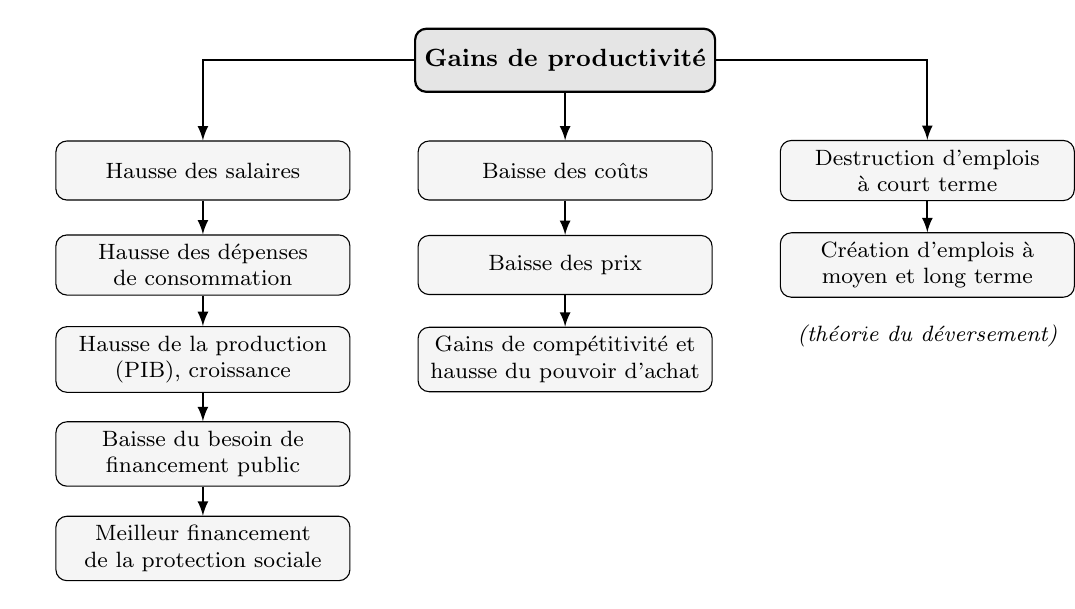
\begin{tikzpicture}[>=latex, every node/.style={font=\footnotesize},
      maillon/.style={draw, rounded corners, align=center, text width=3.5cm,
        minimum height=0.75cm, fill=gray!8,
        execute at begin node={\hyphenpenalty=10000\relax}},
      chaine/.style={->, thick}]
    \node[draw, thick, rounded corners, fill=gray!20, font=\small\bfseries,
      minimum height=0.8cm] (g) at (0,0) {Gains de productivité};
    % chaîne 1
    \node[maillon] (a1) at (-4.6,-1.4) {Hausse des salaires};
    \node[maillon] (a2) at (-4.6,-2.6) {Hausse des dépenses de consommation};
    \node[maillon] (a3) at (-4.6,-3.8) {Hausse de la production (PIB), croissance};
    \node[maillon] (a4) at (-4.6,-5.0) {Baisse du besoin de financement public};
    \node[maillon] (a5) at (-4.6,-6.2) {Meilleur financement de la protection sociale};
    % chaîne 2
    \node[maillon] (b1) at (0,-1.4) {Baisse des coûts};
    \node[maillon] (b2) at (0,-2.6) {Baisse des prix};
    \node[maillon] (b3) at (0,-3.8) {Gains de compétitivité et hausse du pouvoir d'achat};
    % chaîne 3
    \node[maillon] (c1) at (4.6,-1.4) {Destruction d'emplois à court terme};
    \node[maillon] (c2) at (4.6,-2.6) {Création d'emplois à moyen et long terme};
    \node[align=center, font=\footnotesize\itshape] at (4.6,-3.5)
      {(théorie du déversement)};
    \draw[chaine] (g.west) -| (a1.north);
    \draw[chaine] (g.south) -- (b1.north);
    \draw[chaine] (g.east) -| (c1.north);
    \foreach \u/\v in {a1/a2, a2/a3, a3/a4, a4/a5, b1/b2, b2/b3, c1/c2}
      \draw[chaine] (\u.south) -- (\v.north);
  \end{tikzpicture}
  \caption*{\small Les impacts des gains de productivité. The three chains run
    side by side: the first through demand and the public accounts, the second
    through prices, the third through employment, where the jobs destroyed à court terme
    are recreated à moyen et long terme.}
\end{figure}

\paragraph{Désindustrialisation en France.}
The levers work against one structural trend. La part de l'industrie
manufacturière dans le PIB français a baissé de 9 points en quarante ans~: c'est
la \textbf{désindustrialisation} (\textit{deindustrialisation}). Cette évolution
s'explique surtout par le progrès technique et les préférences des
consommateurs~; le commerce extérieur n'a joué qu'un rôle secondaire. La
consommation et l'investissement se sont orientés vers les services. The
manufactured share of household consumption fell from about 52~\% in 1975 to
about 38~\% in 2015, and that of investment excluding construction from about
61~\% to about 39~\%. De même, les dépenses de services par la branche
manufacturière ont augmenté.

\paragraph{Industrial Acceleration Act de 2026 en Europe.}
The European Union's answer, in 2026, is a law with conditions attached:
\begin{itemize}
  \item loi visant à réindustrialiser le continent en conditionnant les
    subventions aux entreprises de secteurs jugés stratégiques, comme
    l'automobile, les technologies d'énergie ou les industries lourdes~;
  \item pour pouvoir bénéficier de fonds publics, les sociétés devront utiliser
    un minimum de composants critiques fabriqués en Europe~: c'est un alignement
    sur les autres pays (par exemple, l'interdiction d'aller sur le marché
    chinois sans un partenaire chinois~; idem aux États-Unis, sur un certain
    nombre de marchés considérés comme appartenant à la sécurité nationale).
\end{itemize}

\paragraph{Réindustrialisation \& décarbonation~: des challenges connectés.}
Bringing production home also cuts emissions. Les importations françaises
représentent 39~\% de l'empreinte carbone du pays. Relocaliser la production
émettrait 40~\% de moins qu'en Asie~; deux règlements européens pénalisent les
importations carbonées~:
\begin{itemize}
  \item le \textbf{Mécanisme d'Ajustement Carbone aux Frontières}
    (\textit{Carbon Border Adjustment Mechanism}, MACF), adopté en 2023, prévoit de
    taxer les importations sur la base de leur contenu carbone dès janvier
    2026~;
  \item le règlement batteries (2023) exclura du marché européen les batteries
    fabriquées dans des pays qui n'ont pas engagé la décarbonation de leur mix
    électrique.
\end{itemize}

\paragraph{Croissance, productivité, emploi, chômage.}
Growth helps the public accounts most when it also brings the chômage down,
and that takes a minimum pace. La croissance ne fait diminuer le taux de
chômage que si elle dépasse un seuil critique, estimable avec la loi d'Okun.

\begin{definition}[Loi d'Okun (\textit{Okun's law})]
  La loi d'Okun (1962) décrit une relation linéaire empirique entre le taux de
  croissance (du PIB) et la variation du taux de chômage. En dessous d'un
  certain seuil de croissance, le chômage augmente~; au-dessus de ce seuil, il
  diminue, à élasticité constante. Elle permet aux économistes de prévoir les
  effets d'un taux de croissance donné sur le chômage. Avec $\bar{Y}$ la
  \textbf{production potentielle} (\textit{potential output}), $Y$ la
  production réelle, $\bar{u}$ le \textbf{taux de chômage naturel}
  (\textit{natural rate of unemployment}), taux d'équilibre à long terme, et
  $u$ le taux de chômage réel~:
  \[ \frac{\bar{Y} - Y}{\bar{Y}} = c\,(u - \bar{u}). \]
\end{definition}

\begin{notation}
  Here $\bar{Y}$, the production potentielle, is the PIB potentiel defined above,
  so $Y - \bar{Y}$ is the écart de production. $c$ is the coefficient of the loi
  d'Okun. In chapter 7 the same letter
  is the propension marginale à consommer of the modèle keynésien; the two
  never meet in one formula.
\end{notation}

\begin{example}[La loi d'Okun aux États-Unis]
  The US estimate is that each point of growth of the PIB above 3~\% lowers
  the taux de chômage by 0,5 point, and each point below 3~\% raises it by as
  much. Aux États-Unis, l'augmentation de 4~\% du PIB effectif réduit donc le
  taux de chômage de $0{,}5 \times (4 - 3) = 0{,}5$ point de pourcentage.
\end{example}

Deux éléments sont critiques, le seuil critique et le coefficient~: ils
évoluent dans le temps et diffèrent selon les pays. The threshold itself has two
sources:
\begin{itemize}
  \item premièrement, la population active n'est pas stable. Si elle croît, par
    exemple, à un taux de 1~\% par an, il est nécessaire que le nombre
    d'emplois progresse à un rythme identique pour que le taux de chômage reste
    constant~: le taux de croissance de la production doit lui aussi être d'au
    moins 1~\%~;
  \item d'autre part, la productivité du travail s'accroît chaque année. La
    production économique doit donc avoir un taux de croissance identique à
    celui de la productivité pour que le taux de chômage reste constant. En
    dessous de ce taux de croissance, les gains de productivité détruisent des
    emplois~; au-dessus, l'économie crée des emplois.
\end{itemize}

\begin{example}[Le seuil de croissance aux États-Unis]
  Si les gains de productivité sont de 1,3~\% par an et que la population
  active augmente de 1,7~\%, comme aux États-Unis, la production doit croître de
  \[ (1{,}013)(1{,}017) - 1 \approx 3~\% \]
  pour maintenir stable le taux de chômage. Au-dessus de ce seuil, la croissance
  de la production dépasse l'augmentation de la production potentielle, et le
  taux de chômage baisse. This is the 3~\% of the estimate above.
\end{example}

Bilan~: le chômage baisse si la croissance effective dépasse la croissance
potentielle (il faut alors embaucher pour dépasser les capacités maximales et
éviter que la demande excède l'offre sur le marché des biens).

\subsection{Conclusion}

The guiding question of the chapter can now be answered.

\begin{example}[Comment réduire le déficit public et stabiliser la dette publique en maintenant la croissance économique~?]
  Four principles sum up the answer:
  \begin{itemize}
    \item \textbf{solidarité}~: faire des économies et des contributions à tous
      les niveaux, par tous les Français, en prenant en compte les effets sur la
      croissance, les emplois et les inégalités~;
    \item \textbf{crédibilité}~: communiquer clairement et avec crédibilité sur
      les scénarios (les articulations des variables et pas seulement les
      montants), sur les recettes anticipées et les usages des ressources, et sur
      le désendettement, pour donner de la crédibilité à une politique de rigueur
      et faire accepter les réformes~;
    \item \textbf{stabilité}~: stabilité politique et engagement sur le long
      terme, pour réduire les incertitudes tant pour les investisseurs que pour
      la croissance économique (il faut agir vite, du fait de l'effet boule de
      neige)~;
    \item \textbf{souveraineté et protection face aux chocs extérieurs} (et
      meilleures anticipations et réactions).
  \end{itemize}
\end{example}

\begin{example}[Une dette publique élevée est-elle toujours un signe d'instabilité~?]
  Non, car la soutenabilité dépend du coût de son service (le taux d'intérêt),
  de la capacité du pays à générer de la croissance (le PIB), de la destination
  des fonds empruntés (investissements productifs ou dépenses courantes) et de
  la démographie. Un pays peut avoir une dette élevée et stable si les
  conditions de financement sont favorables et que la dette génère des retours
  économiques.
\end{example}
